\documentclass[12pt]{kiarticle}
\graphicspath{{pictures/}}
\DeclareGraphicsExtensions{.pdf,.png,.jpg,.eps}
%%%
\pagestyle{fancy}
\fancyhf{}
%\renewcommand{\headrulewidth}{ 0.1mm }
\renewcommand{\footrulewidth}{ .0em }
\fancyfoot[C]{\texttt{\textemdash~\thepage~\textemdash}}
\fancyhead[L]{Вопрос по выбору --- основы современной физики, 2019\hfil}
\fancyhead[R]{\hfil Иванов Кирилл, 625 группа }
\usepackage{multirow} % Слияние строк в таблице
\newcommand
{\un}[1]
{\ensuremath{\text{#1}}}
\usepackage{tikz}
\usepackage{csquotes}
%%% Работа с таблицами
\usepackage{array,tabularx,tabulary,booktabs} % Дополнительная работа с таблицами
\usepackage{longtable}  % Длинные таблицы
\usepackage{multirow} % Слияние строк в таблице
\newcommand{\nbar}{\ensuremath{\overline{n}}}
\newcommand{\ga}{\ensuremath{\gamma}}

\begin{document}
	
	\begin{titlepage}
	\begin{center}
		\large 	Московский физико-технический институт \\
		(национальный исследовательский университет) \\
		Факультет общей и прикладной физики \\
		\vspace{0.2cm}
		
		\vspace{4.5cm}
		Вопрос по выбору в 6 семестре \\ \vspace{0.2cm}
		\large (Основы современной физики) \\ \vspace{0.2cm}
		\LARGE \textbf{Эффект Мессбауэра}
	\end{center}
	\vspace{2.3cm} \large
	
	\begin{center}
		Работу выполнил: \\
		Иванов Кирилл,
		625 группа
		\vspace{10mm}		
		
	\end{center}
	
	\begin{center} \vspace{60mm}
		г. Долгопрудный \\
		2019 год
	\end{center}
\end{titlepage}



\section{Введение}

В данной работе будет обсуждаться вопросы испускания и поглощения атомами твердого тела фотонов (которые возникают при переходе между возбужденными состояниями) и связанный с этим процессом \textbf{эффект Мессбауэра}, заключающийся в бесфононном снятии возбуждения или резонансном поглощении \ga-квантов.

Для сравнения сначала будет кратко описан процесс взаимодействия \ga-квантов и свободных атомов, а затем уже подробно для атомов, закреплённых в кристаллических решетке твердого тела. Будут приведены выкладки для рассчета эффекта Мессбауэра. В завершение работы будет проиллюстрирован эффект резонансного поглощения \ga-лучей на примере возбужденных ядер олова $ ^{119} $ Sn в соединении BaSnO$_3$ при комнатной температуре. Экспериментальные результаты были получены автором в ходе выполнения лабораторной работы № 5.6.1 в 5 семестре. 

\section{Испускание и поглощение в свободных атомах}

	\begin{wrapfigure}[17]{l}{0.35\linewidth}
	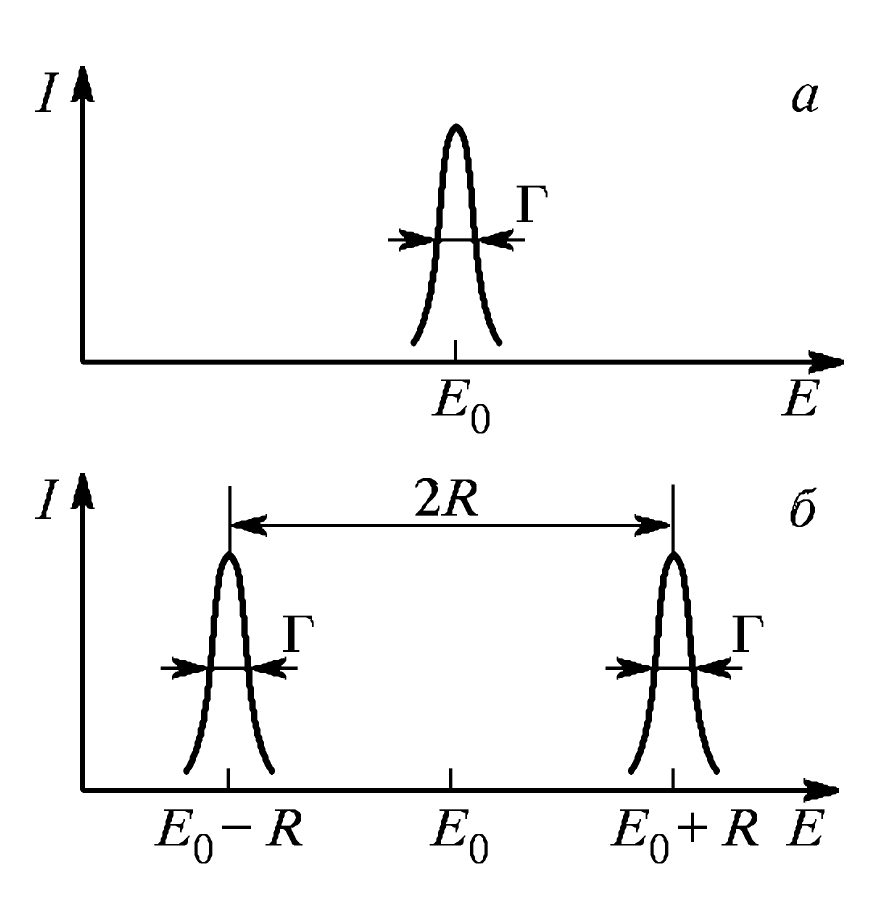
\includegraphics[width=\linewidth]{G}
	\caption{Возбужденное состояние ядра (а),
		и сдвиг линий испускания/поглощения из-за отдачи(б)}
	\label{ris 1}
\end{wrapfigure}

Известно, что атомы могут находится в возбужденных состояниях на определенных (дискретных уровнях), и при переходе из одного состояния в другое они испускают или принимают квант энергии (или же фотон, он же \ga-квант), равный разности энергий между уровнями. При этом в силу принципа неопределённости возбужденные уровни имеют конечную ширину $ \Gamma \simeq \hbar 
\tau $. 

При испускании (поглощении) фотона с импульсом $ p_\ga \hm{=} E_\ga / c $ ядро приобретает в силу ЗСИ импульс $ p_я = p_\ga $ и энергию отдачи $ R $ 

\begin{equation}\label{eq R}
R = \dfrac{P_я^2}{2M_я} = \dfrac{E_\ga^2}{2M_я c^2}
\end{equation}

В силу того, что обычно $ E_\ga $ порядка десятков-сотен кэВ, а масса ядер измеряется в ГэВ, энергия отдачи оказывается порядков мэВ. Однако в силу малости $ \Gamma $  сдвинутые линии не перекрываются (рис. \ref{ris 1}б). 

\begin{wrapfigure}[10]{l}{0.35\linewidth}
	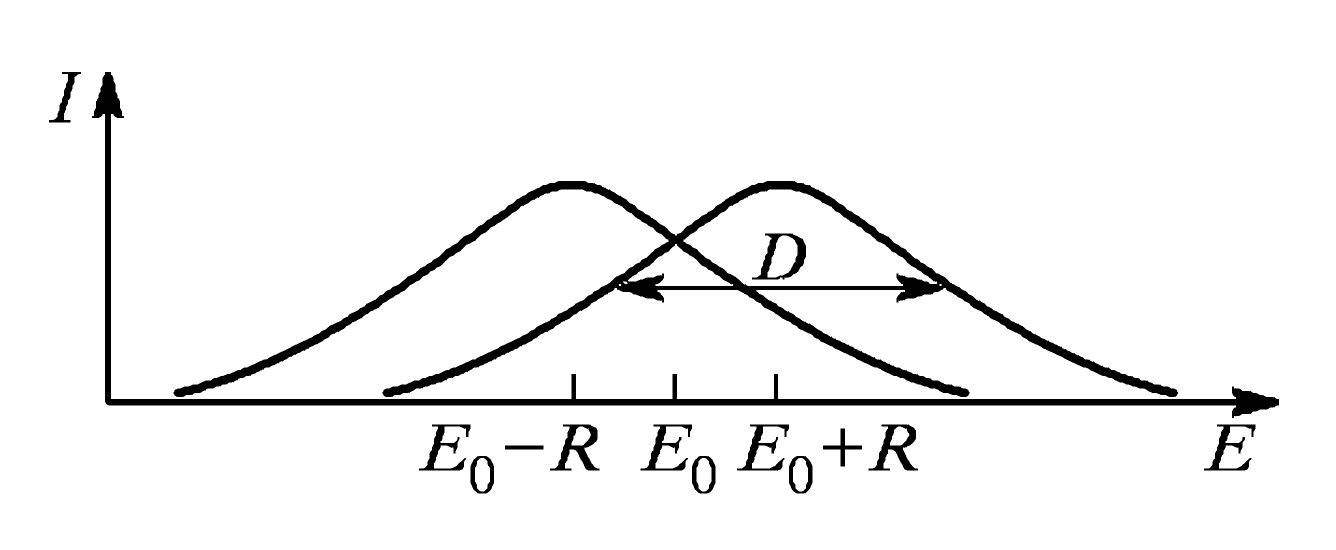
\includegraphics[width=\linewidth]{dopler}
	\caption{Перекрытие линий в силу доплеровского уширения}
	\label{ris dopler}
\end{wrapfigure}

При перекрытии же происходит как раз резонансное поглощение: проходя через невозбужденные атомы, \ga-излучение соответствующей частоты переводит атомы в возбужденное состояние, которое затем испускает фотоны той же частоты. Однако сдвиг энергии отдачи не позволяет этому происходить.

В случае движении испускающих и поглощающих атомов со скоростью $ v = c \x 2R / E_\ga $ происходит доплеровское уширение линии $ D = E\ga \x v/c $ (рис. \ref{ris dopler}). Приведем численные оценки для ядра олова $ ^{119} $ Sn: 

$
E_0 \approx E_\ga = 23,8 \; кэВ, \quad R \approx 2,5 \x 10^{-3} \; эВ, \quad v \hm{\simeq} 60 \; м/с, \quad D \approx 1,5 \x 10^{-2} эВ, \quad \Gamma \simeq 3 \x 10^{-8} \; эВ
$

Таким образом, фотоны с энергией, попадающей в область перекрытия линий, могут создавать резонансное поглощение в свободных атомах. 

\section{Испускание и поглощение в твердых телах}

\subsection{Качественное объяснение}

В случае взаимодействия фотонов с атомами, закреплёнными в кристаллической решетке, при поглощении или испускании фотонов импульс отдачи передается всему твердому телу как целому (считая, что энергия отдачи много меньше энергии связи). В силу этого возникают колебания решетки и рождение квантов этих колебаний --- фононов. 

\textbf{Эффект Мессбауэра состоит в том, что при низких температурах и не очень больших энергиях возможно поглощение (испускание) фотонов без рождения фотонов.} В таком случае энергия отдачи передается всему кристаллу, и в силу обратной пропорциональности массе мы получаем несмещенные линии испускания/поглощения.

В 2000 году в журнале Hyperfine Interactions[3] Мессбауэр привёл такую наглядную интерпретацию эффекта:

\begin{displayquote}
	\textit{Ситуация … напоминает человека, прицельно бросающего камень из лодки. Большую часть энергии согласно закону сохранения импульса получает лёгкий камень, но небольшая часть энергии броска переходит в кинетическую энергию получающей отдачу лодки. Летом лодка просто приобретёт некоторое количество движения, соответствующее отдаче, и отплывёт в направлении, противоположном направлению броска. Однако зимой, когда озеро замерзнет, лодку будет удерживать лёд, и практически вся энергия броска будет передана камню, лодке (вместе с замерзшим озером и его берегами) достанется ничтожная доля энергии броска. Таким образом, отдача будет передаваться не одной только лодке, а целому озеру, и бросок будет производиться «без отдачи».}
\end{displayquote} 

\subsection{Вычисление вероятности эффекта}

Рассмотрим, как это происходит. В модели твердого тела Эйнштейна будем считать, что каждый атом колеблется независимо, подобно гармоническому осциллятору в потенциальной яме, образованной силой взаимодействия с соседями по решетке. В таком случае спектр возбуждений кристалла --- уровни $ E_n = (n + 1/2) E_Д $, т.е. эти колебания распостраняются квантами-фононами с дебаевской энергией 

\begin{equation}\label{}
E_Д = \hbar \omega_Д = \pi \hbar s / a = k_Б \Theta
\end{equation} 

где параметры кристалла: $ s $ --- скорость звука, $ a = \lambda_Д/2 $ --- расстояние между атомами, $ \Theta = \hbar s k_Д $ --- температура Дебая. Процесс взаимодействия с \ga-квантом можно интерпретировать как случаный, в ходе которого вероятность случайной величины (переданной энергии в размере $ n $ фононов ) распределена по Пуассону в силу независимости событий:

\begin{equation}\label{eq puasson}
P(n) = \dfrac{\mu^n}{n!} e^{-\mu}
\end{equation}

Параметр $ \mu $ --- среднее число событий за заданный период времени --- в нашем случае равен среднему числу квантов колебаний с энергией $ \hbar \omega_Д  $, возбужденных энергией отдачи $ R $, т.е. $ \mu \hm{=} \dfrac{R}{\hbar \omega_Д} $. Нас интересует вероятность события, в котором родилось $ n = 0 $ фононов, т.е. 

\begin{equation}\label{eq P(0)}
f = P(0) = \exp \left( - \dfrac{R}{\hbar \omega_Д} \right) 
\end{equation}

Преобразуем это выражение в следующий вид. Для частицы с массой $ M $, колеблющейся с частотой $ \omega $, потенциальная энергия 

\begin{equation}\label{}
\langle U \rangle = \dfrac{1}{2} M \omega^2 \langle u^2 \rangle = \langle K\rangle = \dfrac{1}{2} E_0 = \dfrac{1}{4} \hbar \omega \te \left\langle u^{2}\right\rangle=\dfrac{\hbar}{2 M \omega}
\end{equation} 

Здесь $  \langle u^2 \rangle $ --- среднеквадратичное смещение, а для равенства $ U = K = E/2 $ была использована теорема вириала. Подставив \eqref{eq R} вместо $ R $ в формулу \eqref{eq P(0)} и заменив $ \lambda=2 \pi \hbar c / E_{\gamma} $, мы получаем 

\begin{equation}\label{f =}
\dfrac{R}{\hbar \omega_Д} = \frac{E_{\gamma}^{2}}{2 M c^{2} \hbar \omega_{Д}}=\frac{E_{\gamma}^{2}}{\hbar^{2} c^{2}} \frac{\hbar}{2 M \omega_{Д}}=4 \pi^{2} \frac{\left\langle u^{2}\right\rangle}{\lambda^{2}} \te f = \exp \left( - 4 \pi^{2} \frac{\left\langle u^{2}\right\rangle}{\lambda^{2}}  \right) 
\end{equation}

Из этого выражения следует, что вероятность излучения кванта
без потери на возбуждение колебаний решетки (рождения фононов)
велика тогда, когда амплитуда колебаний атома в решетке мала по
сравнению с длиной волны излучаемого ядром \ga-кванта. Понятно, что амплитуда колебаний пропорциональна температуре, а длина волны \ga-кванта обратна его энергии. Этим и обусловлены условия, при котором вероятность эффекта Мессбауэра $ f $ велика: низкие температуры и не слишком большие энергии фотонов.

\subsection{Рассмотрение зависимости от температуры}

Попробуем получить более явную зависимость от температуры в общем случае. В самом деле, запишем теорему вириала в виде

\begin{equation}\label{}
E_n = \hbar \omega (k) \left( n(k) + \dfrac{1}{2} \right)  = 2 \langle U \rangle = M \omega^2 \langle u^2 \rangle
\end{equation}

C учетом того, что фононы --- бозоны с тремя поляризациями (одна продольная и две поперечных), в модели $ \omega = sk $ мы получаем 

 \begin{equation}\label{}
  \langle u^2 \rangle = 3 V_я \int \dfrac{d^3 \mathbf{k}}{ (2 \pi)^3} \dfrac{\hbar}{sk M} \left( \dfrac{1}{\exp ( \frac{\hbar \omega}{k_БT} )- 1 } + \dfrac{1}{2} \right) = 3 V_я  \int\limits_0^{k_Д} \dfrac{k^2\, dk}{2 \pi^2} \dfrac{\hbar}{sMk} \left( \dfrac{1}{\exp ( \frac{\hbar s k}{k_БT} )- 1 } + \dfrac{1}{2} \right) 
   \end{equation}
   
   Сделав в первом члене замену $ x = \frac{\hbar s k}{k_БT} $, мы получаем 
   
   \begin{equation}\label{}
   \langle u^2 \rangle = \dfrac{3V_я}{2\pi^2 sM} \left( \dfrac{k_Б^3T^3}{\hbar^2 s^3} \int\limits_0^{\frac{\hbar s k_Д}{k_БT}} \dfrac{x \, dx}{e^x - 1} + \dfrac{\hbar k_Д^2}{4} 
   \right) 
   \end{equation}
   
   Таким образом, мы видим, что действительно амплитуда колебаний пропорциональная температуре в силу первого члена, и при низких температурах мы можем получить (пользуясь $ \dfrac{(2\pi)^3}{V_я}  = \dfrac{4}{3} \pi k^3_Д$)
   
   \begin{equation}\label{}
   \langle u^2 \rangle \xrightarrow{T \st 0}  \dfrac{3 \x 6\pi^2  \hbar k^2_Д}{8\pi^2 sM k^3_Д} = \dfrac{9\hbar^2}{4 M k_Б \Theta}
   \end{equation}
   
   Подставляя это в наше выражение для эффекта Мэссбауэра \eqref{f =} и возвращаясь к энергии $ E_\ga $, мы получаем 
   
   \begin{equation}\label{}
   f = \exp \left( - \dfrac{3}{4} \dfrac{E^2_\ga }{Mc^2 k_Б\Theta}  \right) 
   \end{equation}
   
   В задании была задача Т.5 для кристалла $ ^{193} $ Ir с энергией \ga-кванта $ E_\ga = 129 \; кэВ, \; \Theta = 430 \; К $. Можно получить максимальную вероятность эффекта $ f \approx 15 \% $. 
   
   Если же не пользоваться приближение низких температур и оценить средную амлитуду колебаний просто из теплового движения 
   
   \begin{equation}\label{}
    \langle u^2 \rangle \simeq \dfrac{k_БT}{M \omega_{Д}} \te f = \exp \left( - \dfrac{E^2_\ga}{Mc^2} \dfrac{T}{k_Б \Theta^2} \right) 
   \end{equation}
   
   \section{Экспериментальное наблюдение эффекта}
   
   \subsection{Описание работы}
   
   В лабораторной работе № 5.6.1. изучается эффект Мессбауэра следующим образом. \ga-излучение возбужденных ядер $ ^{119} $ Sn соединения BaSnO $_3$ пропускается через резонансный поглотитель со стабильными ядрами $ ^{119} $ Sn. Пройдя через него, излучение регистрируется сцинтилляционным спектрометром.  
   
   Наблюдение резонансного поглощения основано на методе доплеровского сдвига линий испускания и поглощения. Для этого поглотителю придается небольшая скорость $ v = c \x 2 \Gamma / E_\ga $. Мессбауэровская линия очень узка, и для наблюдения резонанса хватает скорости порядка миллиметра в секунду. 
   
   \begin{figure}[h!]
   	\centering
   	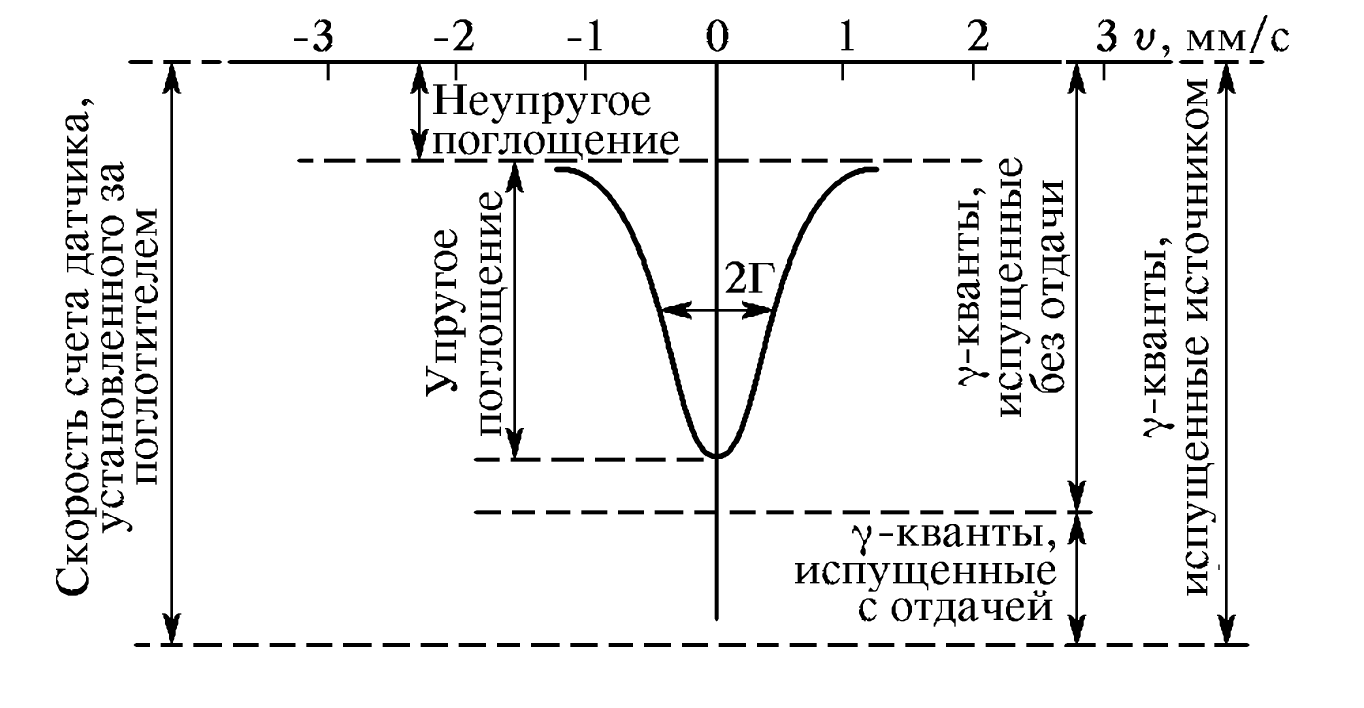
\includegraphics[width=0.7\linewidth]{spektr}
   	\caption{Спектр упругого резонансного поглощения $ \gamma $-квантов. Источник и поглотитель находятся в идентичных кристаллических решетках. Неупругое поглощение
   		обусловлено главным образом взаимодействием $ \gamma $-лучей с атомными электронами}
   	\label{ris 2}
   \end{figure}
   
   Вообще говоря, при идентичных кристаллических решетках, линия испускания полностью перекрывается с линией поглощения, и максимальное поглощение наблюдается при нулевой скорости (рис. \ref{ris 2}). Однако в химических сплавах (как наш BaSnO$_3$) из-за влияния электростатических сил происходит смещение максимума поглощения, и его можно "<поймать"> при отличной от нуля скорости. Такое смещение называется \textbf{химическим сдвигом}. Его можно рассчитать по формуле 
   
   \begin{equation}\label{vr}
   v_p = \dfrac{\Delta E}{E_0}c
   \end{equation}
   
   Для подсчета "<амплитуды"> эффекта Мессбауэра определяется безразмерная величина
   
   \begin{equation}\label{epsi;on}
   \epsilon(v) = \dfrac{N (\infty) - N(v)}{N (\infty) - N_ф}
   \end{equation}
   
   где $ N(v) $ --- скорость счета квантов, прошедших через поглотитель при
   некоторой скорости $ v $, $ N (\infty) $ --- скорость счета квантов при достаточно
   большой скорости, когда резонансное поглощение отсутствует, $ N_ф  $ --- скорость счета радиоактивного фона.
   
   Измеряемая на опыте ширина резонансной линии $  \Gamma_{экс} $ --- результат наложения линий источника и поглотителя. При тонких поглотителях и источниках и при отсутствии вибраций ширина линии равна удвоенной естественной ширине $ 2\Gamma $ (см. рис. \ref{ris 2}).
   
   На рис. \ref{ris 2} кривая задается формулой Брейта-Вигнера (лоренцева кривая):
   
   \begin{equation}\label{B-V}
   \sigma(E) \propto \dfrac{(\Gamma/2)^2}{(E - E_0)^2 + (\Gamma/2)^2}
   \end{equation}
   
   \subsection{Экспериментальные результаты для разных поглотителей}
   
   Быри проведены измерения резонансного поглощения на 4-ех образцах: №1, №2, №3 --- это олово разной толщины, а №4 --- SnO$ _2 $. Экспериментальные точки и их фиты приведены на графиках. Результаты всех 4-ех фитов сведем в таблицу \ref{table_fit}.
   
     \begin{figure}[H]
   	\label{graf_1}
   	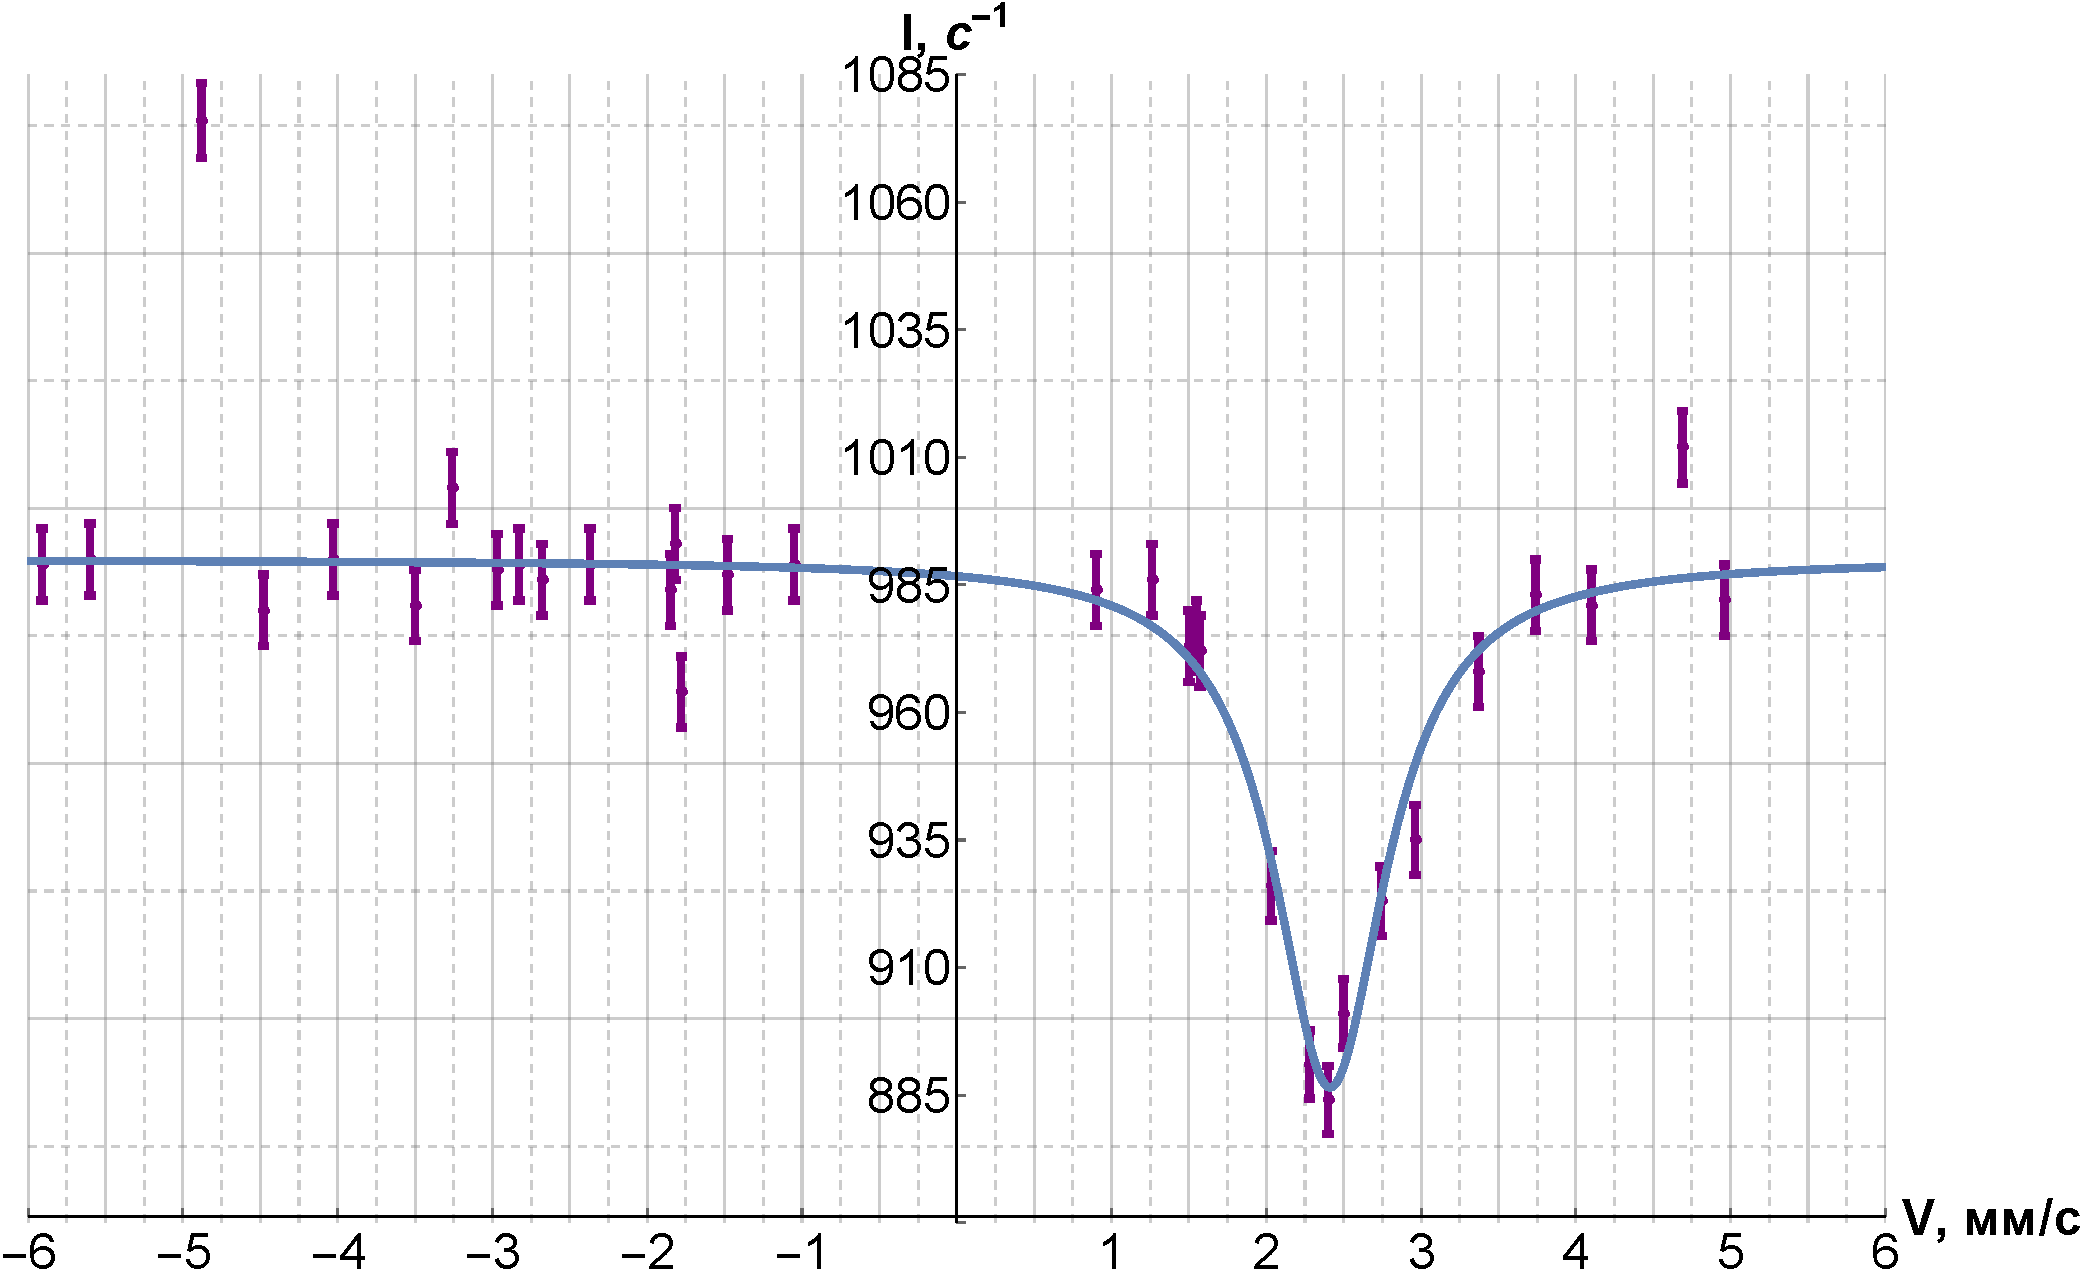
\includegraphics[scale=0.47]{gr1.pdf}
   	\caption{Резонансное поглощение на 1-ом поглотителе}
   \end{figure}
   
   \begin{figure}[H]
   	\label{graf_2}
   	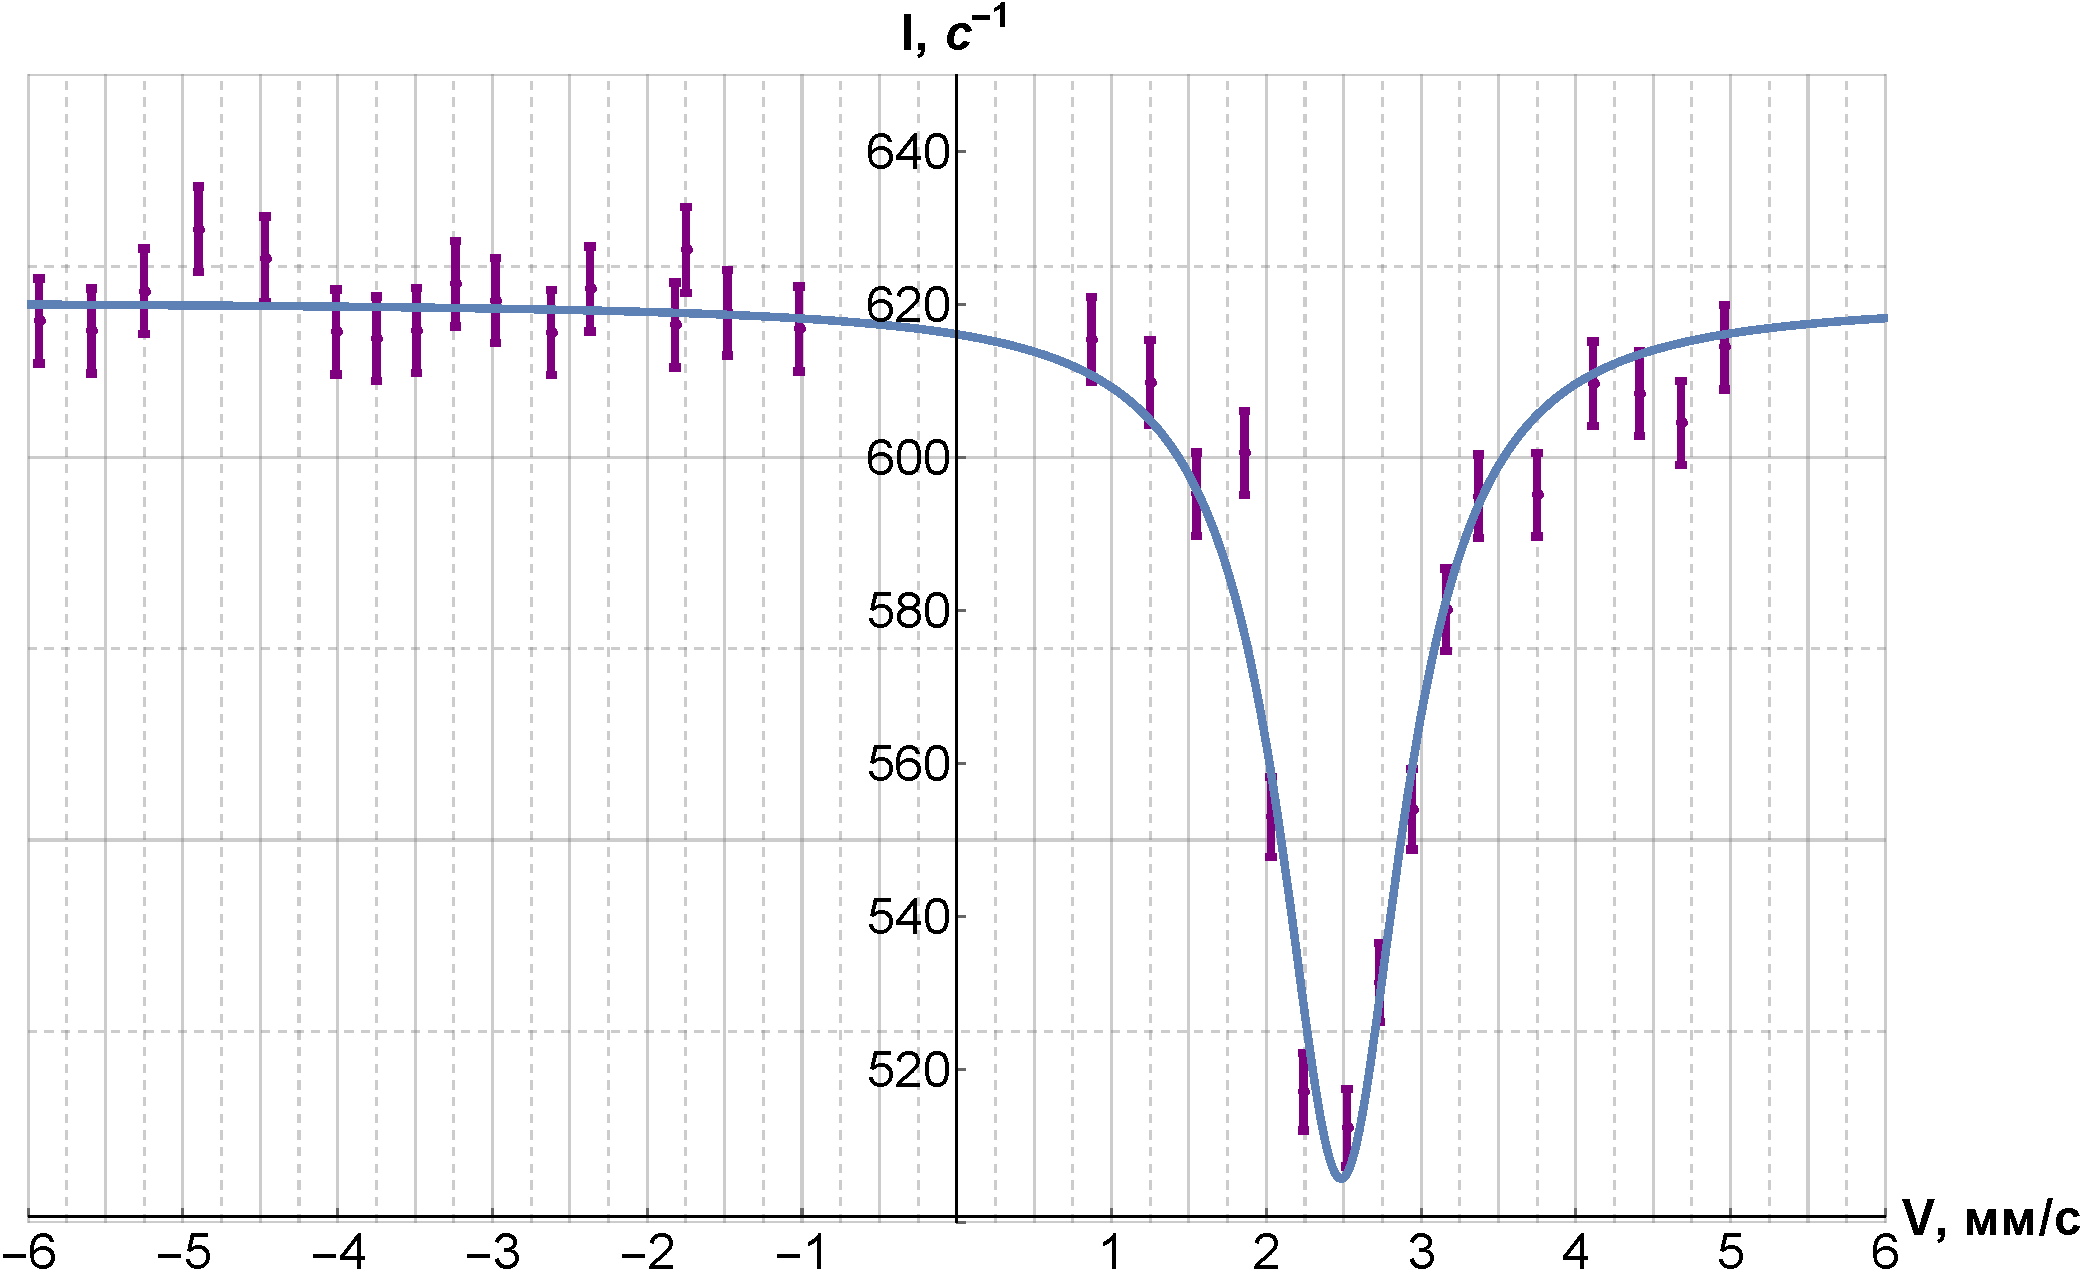
\includegraphics[scale=0.47]{gr2.pdf}
   	\caption{Резонансное поглощение на 2-ом поглотителе}
   \end{figure}
   
   \begin{figure}[H]
   	\label{graf_3}
   	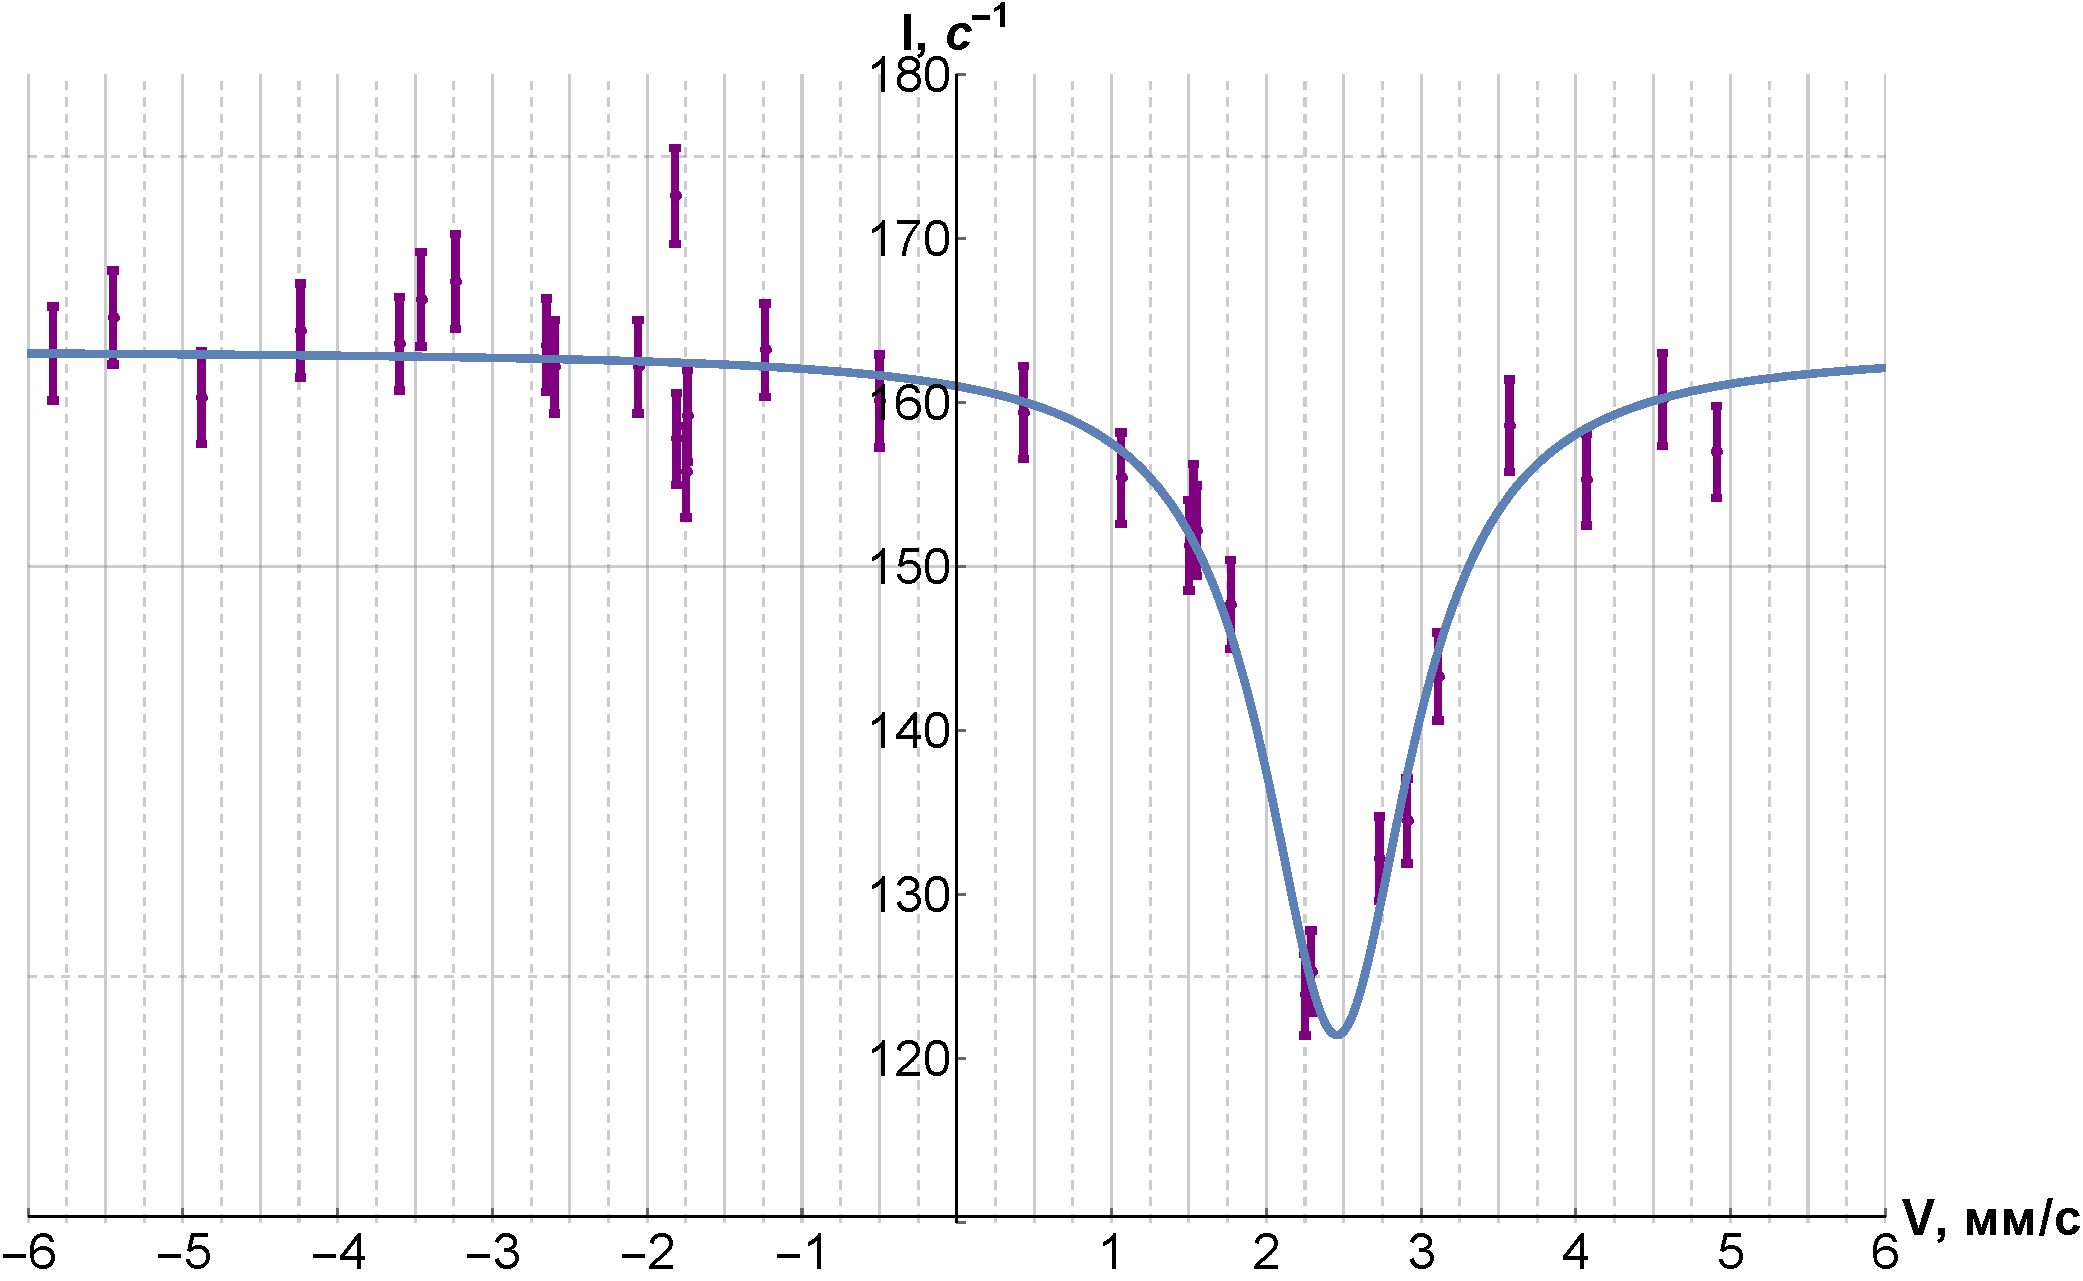
\includegraphics[scale=0.47]{gr3.pdf}
   	\caption{Резонансное поглощение на 3-ом поглотителе}
   \end{figure}
   
   \begin{figure}[H]
   	\label{graf_4}
   	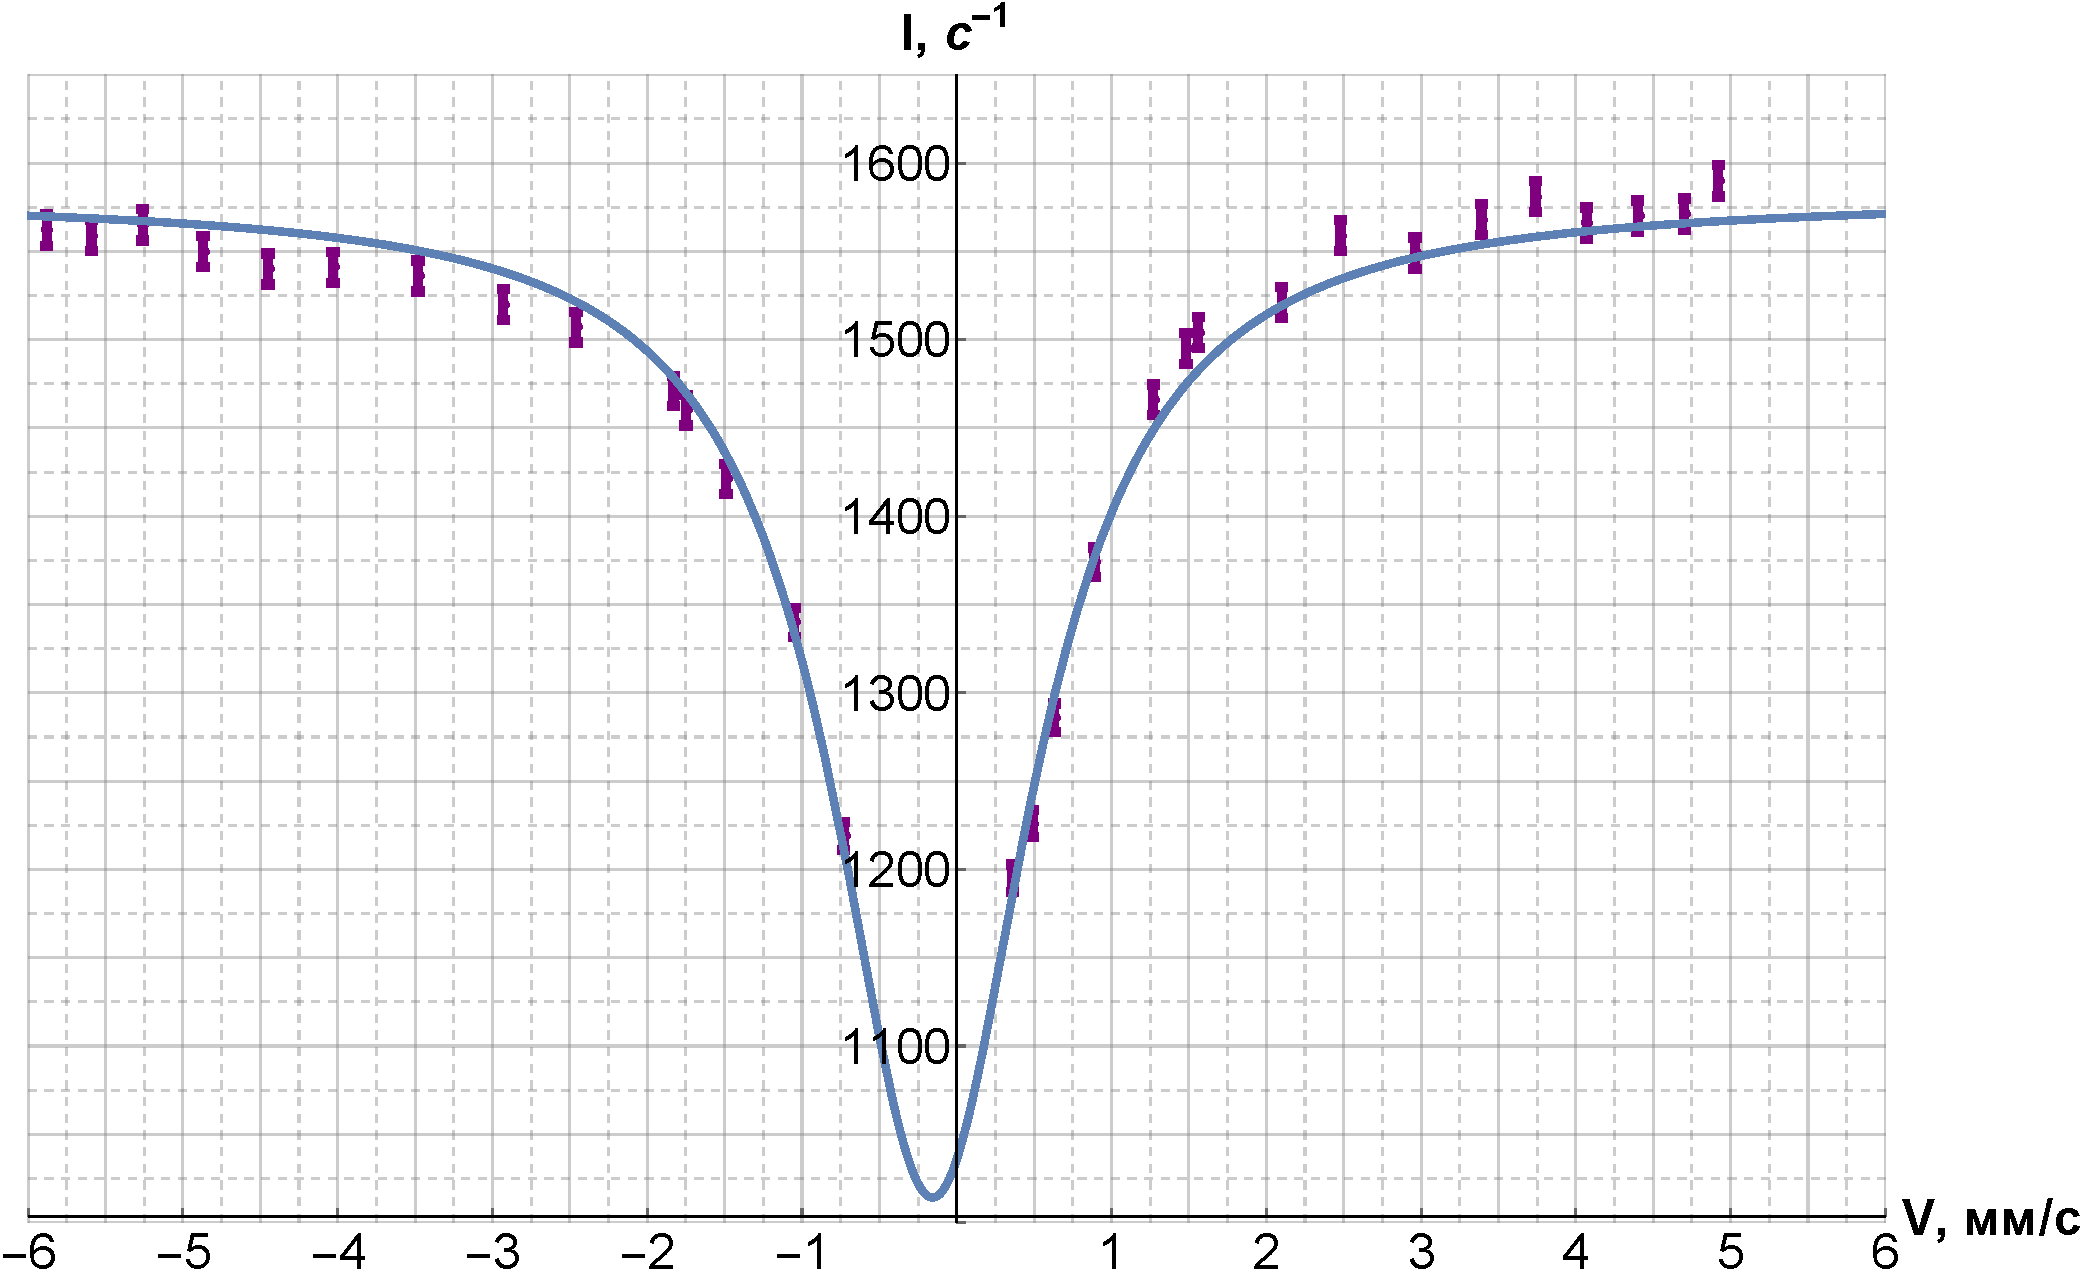
\includegraphics[scale=0.47]{gr4.pdf}
   	\caption{Резонансное поглощение на 4-ом поглотителе}
   \end{figure}
   
   \begin{table}[h]
   	\caption{Результаты фитирования кривой резонансного поглощения}
   	\begin{center}
   		\begin{tabular}{|c|c|c|c|c|c|}
   			\hline
   			$ № $&  $ a  $ & $ b, \; с^{-1} $,  &  $ c, мм/c $ & $ X, мм/с $ & $ \chi_\nu^2 $ \\
   			\hline
   			1 & $ 103 \pm 6 $ & $ 990\pm 4 $ & 0,43 $\pm $ 0,04& $ 2,41 \pm 0,03 $ & 1,68 \\
   			2 & 114 $  \pm 5$ & \text{620 $  \pm $ 3} & \text{0,49 $  \pm $ 0,04} & \text{2,48 $ \pm $ 0,02} & 1,59\\
   			3 & \text{41 $  \pm  $ 3} & \text{163 $  \pm $ 1} & \text{0,58 $  $$ \pm $ 0,06} & \text{2,46 $ $$ \pm $ 0,03} & 1,43 \\
   			4 & \text{566$  $$ \pm $ 31} & \text{1580$  $$ \pm $ 5} & \text{0,78$  $$ \pm $ 0,05} & \text{-0,156$ 
   				$$ \pm $ 0,015} & 2,63\\
   			\hline
   		\end{tabular}
   	\end{center}
   	\label{table_fit}
   \end{table}
   
   В полученных параметрах фита: $ b $ --- величина фона, из которого мы "<вычитаем"> мэсбауэровский пик, $ 2с $ --- ширина резонансной линии $ \Gamma_{экс} $, а $ X $ --- величина химического сдвига. Под $ \chi_\nu^2 $ имеется ввиду критерий $ \chi^2 $, отнесенный к числу степеней свободны.
   
   На основе полученных результатов фитов мы можем вычислить амплитуды поглощения по формуле \eqref{epsi;on}. 
   
   С учетом того, что $ N(\infty) = b, \; N(v) = y(X) $, мы можем подсчитать искомую величину. По формуле $ \Gamma_{экс} =  E_\gamma \x v/c $ мы можем оценить ширину уширения линии $  \Gamma_{экс} $ в эВ, подставляя как $ v = 2с , E_\gamma = 23,8 $ кэВ ($ c $ --- параметр фита).  Также из \eqref{vr} мы можем подсчитать химический сдвиг $ \Delta E $ в эВ, подставляя в качестве $ v_r = X $.  Вычисление параметров для всех поглотителей сведено в таблицу.
   
   \begin{table}[h!]
   	\caption{Результаты работы}
   	\begin{center}
   		\begin{tabular}{|c|c|c|c|c|c|}
   			\hline 
   			№ & $\epsilon_i, \%$ & $ \Gamma_{экс}, мм/с $ & $  \Gamma_{экс}, 10^{-8} \x$ эВ & $ v_р, мм/с $ & $ \Delta E, 10^{-7}\x $, эВ \\ 
   			\hline 
   			1 & $ 10,6 \pm 0,9 $ & $ 0,86 \pm 0,08 $  & $ 7,3 \pm 0,6 $ & $ 2,41 \pm 0,03 $ & $ 1,91 \pm 0,02 $ \\ 
   			\hline 
   			2 &  $ 18,9 \pm 1,5 $& $ 0,98 \pm 0,09 $  & $  7,8 \pm 0,7 $ & $ 2,48 \pm 0,02 $ & $  1,97 \pm 0,01 $ \\ 
   			\hline 
   			3 & $ 28,1 \pm 0,9 $ & $ 1,116 \pm 0,12 $ & $  9,2 \pm 0,8 $ & $ 2,46 \pm 0,03 $ &  $ 1,95 \pm 0,02 $\\ 
   			\hline 
   			4 & $ 36,1 \pm 3,2 $  & $ 1,56 \pm 0,11 $ & $ 12,3 \pm 1,3  $ & $ -0,156 \pm 0,015 $ &  $ -0,123 \pm 0,006 $\\ 
   			\hline 
   		\end{tabular} 
   	\end{center}
   	\label{res}
   \end{table}
   
   Полученные результаты соотносятся с теоретическими расчетами. Уширение резонансной кривой по сравнению с $ 2\Gamma= 6\x10^{-8} $ эВ происходит при увеличении ширины поглотителя.
 
   
   
\section*{Использованная литература}

\begin{itemize}
	
	\item[[1]] Лабораторный практикум по общей физике: учеб. пособие. В трёх томах. Т. 2. Оптика / А.В. Максимычев, Д.А. Александров, Н.С. Берюлёва и др.; под ред. А.В. Максимычева. --- М.: МФТИ, 2014. --- 446 с.
	
	\item[[2]]  Ципенюк Ю.М. Квантовая микро- и макрофизика. М.: Физматкнига, 2006. --- 640 c. 
	
	\item[[3]]   Rudolf L. Mössbauer. The discovery of the Mössbauer effect (англ.) // Hyperfine Interactions. — 2010. — Vol. 126. — P. 1—12. — DOI:10.1023/A:1012620106837.
	
\end{itemize}


\end{document}